\documentclass[]{aiaa-tc} %load in aiaa class template file
\usepackage{amsmath}
\usepackage{mathrsfs}
\usepackage{hyperref}
\usepackage{natbib} %REMOVE THIS IF YOU DON'T WANT BRACKETS ON YOUR PAPER
\usepackage{float}
\usepackage{color,soul}
\usepackage[font=normalsize,labelfont=bf]{caption}

\newcommand{\sref}[1]{$^{[\ref{#1}]}$}
\newcommand{\dref}[2]{$^{[\ref{#1}-\ref{#2}]}$}

 \title{\bf Equations of Motion of a Perpetual Motion Device}

 \author{
   Carlos Montalvo\thanks{Assistant Professor, Department of Mechanical
    Engineering, Member AIAA}\\
   {\normalsize\itshape Facility for Aerospace Systems and Technology (FAST)}\\
   {\normalsize\itshape College of Engineering}\\
{\normalsize\itshape
    University of South Alabama, Mobile, AL USA}}
 \date{}

 \linespread{1}

 % Define commands to assure consistent treatment throughout document
\newcommand{\eqnref}[1]{(\ref{#1})}
\newcommand{\class}[1]{\texttt{#1}}
\newcommand{\package}[1]{\texttt{#1}}
\newcommand{\file}[1]{\texttt{#1}}
\newcommand{\BibTeX}{\textsc{Bib}\TeX}

\begin{document}

\maketitle

\begin{abstract}

Here we investigate the equations of motion of a perpetual motion
device.

\end{abstract}

%%%%%%%%%%%%%%%%%%%%%%%%%%%%%%%%%%%%%%%%%%%%%%%%%%%%%%%%%%%%%%%%%%%
%%%%%%%%%%%%%%%%%%%%%%%%%%%%%%%%%%%%%%%%%%%%%%%%%%%%%%%%%%%%%%%%%%%
%%%%%%%%%%%%%%%%%%%%%%%%%%%%%%%%%%%%%%%%%%%%%%%%%%%%%%%%%%%%%%%%%%%

\begin{tabbing}
  XXXXXXXXXX \= \kill% this line sets tab stop
  $x,y,z$ \> components of the mass center position vector in the
  inertial frame (m)  \\
  $\phi,\theta,\psi$ \> Euler roll,pitch, and yaw angles (rad) \\
  $q_0,q_1,q_2,q_3$ \>  Quaternions \\  
  $u,v,w$ \> components of the mass center velocity vector in the
  body frame (m/s)  \\
  $p,q,r$ \> components of the mass center angular velocity vector in the
  body frame (rad/s)  \\
  $\vec{\omega}_{B/I}$ \> Angular velocity vector of the satellite in
  the body frame (rad/s) \\
  ${\bf T}_{IB}$ \> rotation matrix from frame I to frame B \\
  ${\bf H}$ \> relationship between angular velocity components in
  body frame and derivative of Euler angles \\
  $m$ \> mass (kg) \\
  $I$ \> mass moment inertia matrix about the mass center
  in the body frame ($kg-m^2$)  \\
  $X,Y,Z$ \> components of the total force applied to CubeSAT in
  body frame (N)  \\
  $L,M,N$ \> components of the total moment applied to CubeSAT in
  body frame (N-m)  \\
  ${\vec r}_{A\rightarrow B}$ \> position vector from a generic point A
  to a generic point B (m) \\
  ${\vec V}_{A/B}$ \> velocity vector of a generic point A
  with respect to a generic frame B (m/s) \\
  ${\bf S}(\vec{r})$ \> skew symmetric matrix operator on a
  vector. Multiplying this matrix by a vector is equivalent \\
  \> to a cross product\\
 \end{tabbing}

%%%%%%%%%%%%%%%%%%%%%%%%%%%%%%%%%%%%%%%%%%%%%%%%%%%%%%%%%%%%%%%%%%%
%%%%%%%%%%%%%%%%%%%%%%%%%%%%%%%%%%%%%%%%%%%%%%%%%%%%%%%%%%%%%%%%%%%
%%%%%%%%%%%%%%%%%%%%%%%%%%%%%%%%%%%%%%%%%%%%%%%%%%%%%%%%%%%%%%%%%%%


\section{Mathematical Model}

The perpetual motion device presented here is a simple wheel supported by a
triangular structure. The wheel can rotate about its center of
mass. In order to keep energy in the system, rods are located around
the wheel and constrained to move about 30 to 45 degrees. When the rod
moves from its first constrained position to its other constrained
position there is momentum transfer between the rod and the
wheel. This momentum transfer keeps the machine moving.

To derive the equations of motion of this device first the device is
simplified to only have 1 rod and the rod is completely unconstrained
as shown in the figure below. The wheel rotates about point O through
angle $\theta$. The rod is connected and rotates about point C and is
a distance r from the center of the wheel. The rod rotates through
angle $\phi$. The angle $\psi$ is used to prescribe the location of
the connection point C in the wheel's frame of reference.
\begin{figure}[H]
  \begin{center}
    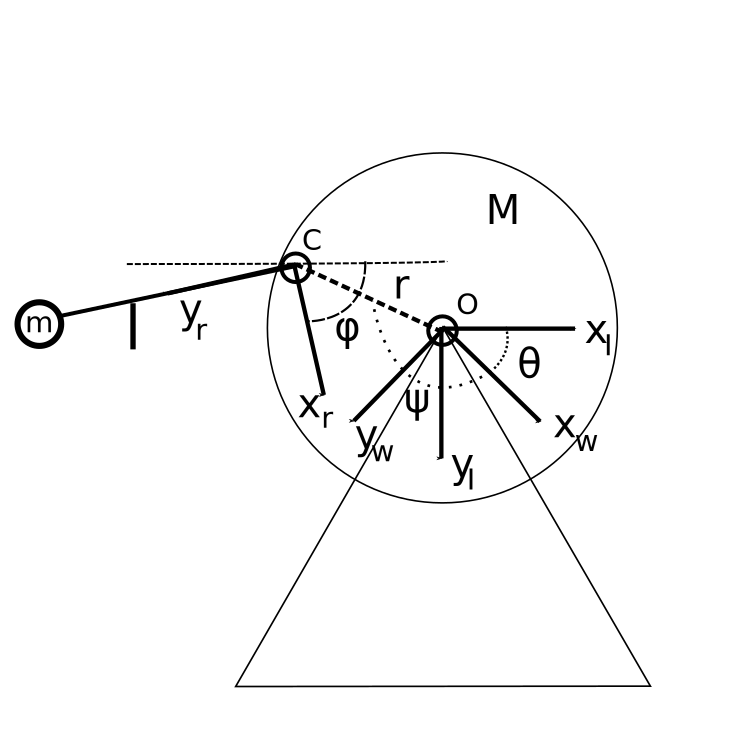
\includegraphics[height=100mm]{Main_Graphic.pdf}
  \end{center}
  \caption{\bf Schematic of Simple Perpetual Motion Machine}
  \label{f:current}
\end{figure}
Three reference frames are used here. The first is the inertial frame
which has $x_I$ pointed to the right and $y_I$ pointed downwards. The
wheel frame (w) rotates with the wheel and the rod frame (r) rotates
with rod. In order to derive the equations of motion Lagrange's method
is used.
\begin{equation}\label{e:lagrangian}
  \frac{d}{dt} \left( \frac{\partial L}{\partial q} \right) - \frac{\partial
    L}{\partial q} = Q_{nc}
\end{equation}
where $L=K-V$ is the Lagrangian and is equal to the Kinetic energy of
the system minus the potential energy of the system. The
non-conservative forces are non-existent since for the moment any
contact between joints is ignored. The variable $q$ is an array of all
the independent variables in the system which in this case is $\theta$
and $\phi$. To start the kinetic energy is written such that the wheel
has rotational energy and the rod only has translational energy. The
rod is assumed to be massless and thus has no rotational energy. 
\begin{equation}
  K = \frac{1}{2}I_w\dot{\theta}^2 +
  \frac{1}{2}m\vec{v}_{m/I}^T\vec{v}_{m/I}
\end{equation}
The velocity of the mass is derived by writing the position of the
mass in inertial coordinates which can be seen as a linear combination
of a vector from the center of mass of the wheel to the edge and then
down the length of the rod. 
\begin{equation}
  \vec{r}_m = r cos(\psi) \hat{x}_w + r sin(\psi) \hat{y}_w + l \hat{x}_r
\end{equation}
Transforming this equation into inertial coordinates results in the
following equation where standard shorthand is for cosine and sine
functions. 
\begin{equation}
  \vec{r}_m = [r (c_{\psi}c_{\theta} - s_{\psi}s_{\theta}) + lc_{\phi}]\hat{x}_I + 
  [r (c_{\psi}s_{\theta} + s_{\psi}c_{\theta})+ls_{\phi}]\hat{y}_I
\end{equation}
Taking a derivative of the equation above yields the velocity of the
mass m in the inertial frame. Note that $r$, $l$ and $\psi$ are
constants.
\begin{equation}
  \vec{v}_{m/I} = -[r(c_{\psi}s_{\theta}+s_{\psi}c_{\theta})\dot{\theta}+ls_{\phi}\dot{\phi}]\hat{x}_I
  + [r(c_{\psi}c_{\theta}-s_{\psi}s_{\theta})\dot{\theta}+lc_{\phi}\dot{\phi}]\hat{y}_I
\end{equation}
The kinetic energy of the end mass is then equal to the norm of the
velocity vector squared time one half the mass. First the square of
the norm of velocity is computed below.
\begin{equation}
  \vec{v}_{m/I}^T\vec{v}_{m/I} =
      [r(c_{\psi}s_{\theta}+s_{\psi}c_{\theta})\dot{\theta}+ls_{\phi}\dot{\phi}]^2
      + [r(c_{\psi}c_{\theta}-s_{\psi}s_{\theta})\dot{\theta}+lc_{\phi}\dot{\phi}]^2
\end{equation}
With the Kinetic energy now known, the potential energy $V$ must be
computed. If the line of zero potential is located at the center of
mass of the wheel and positive potential above it and negative
potential below it the potential energy of the wheel becomes zero. The
potential energy of the mass then simply becomes
\begin{equation}
  V=-mg\vec{r}_m^T\hat{y}_I = -mg[r (c_{\psi}s_{\theta} +
  s_{\psi}c_{\theta})-ls_{\phi}]
\end{equation}
At this point the full Lagrangian $L$ can be written as the following
where the moment of inertia of the wheel is written as $I_w=\frac{1}{2}Mr^2$
\begin{equation}
  L = \frac{1}{4}Mr^2\dot{\theta}^2 + \frac{1}{2}m[r(c_{\psi}s_{\theta}+s_{\psi}c_{\theta})\dot{\theta}+ls_{\phi}\dot{\phi}]^2
      +
      [r(c_{\psi}c_{\theta}-s_{\psi}s_{\theta})\dot{\theta}+lc_{\phi}\dot{\phi}]^2
      + mg[r (c_{\psi}s_{\theta} +
        s_{\psi}c_{\theta})-ls_{\phi}]
\end{equation}
The equation above is extremely long and cumbersome thus the program
Mathematica was used to obtain the equations of motion using equation
\ref{e:lagrangian}. The equation below is extremely non-linear however
extremely simple to simulate using any numerical integration scheme by
simply inverting the inertia matrix and solving for the accelerations
of the wheel and the rod. 
\begin{equation}
  \begin{bmatrix} \frac{1}{2}Mr^2 + mr^2 & l m r cos(\theta-\phi+\psi)
    \\ l m r cos(\theta-\phi+\psi) & m
    l^2 \end{bmatrix}\begin{Bmatrix} \ddot{\theta}
    \\ \ddot{\phi} \end{Bmatrix} = -\begin{Bmatrix} l m r sin(\theta-\phi+\psi) \dot{\phi}^2 + m g r
    sin(\theta+\psi) \\ -l m r
    sin(\theta-\phi+\psi)\dot{\theta}^2 + m g l
    sin(\phi) \end{Bmatrix}
\end{equation}
%% This equation can be written in compact form such that
%% \begin{equation}
%%   I\ddot{q} = -P
%% \end{equation}
The difficulty in determining the equations of motion of this
perpetual motion device stems in the difficulty in writing the result
of the Lagrangian using more than one rod. The equations of motion
form a pattern when increasing the number of rods and can actually be
written in a pretty simple closed form expression as shown below where
$N$ is the number of rods,
$\alpha_i = l_im_ircos(\theta-\phi_i+\psi_i)$, $\beta_i =
l_im_irsin(\theta-\phi_i+\psi_i)$, $\gamma_i=m_igr_isin(\theta+\psi_i)$
and $\delta_i = m_igl_isin(\phi_i)$
\begin{equation}
  \begin{bmatrix} \frac{1}{2}Mr^2 + \sum\limits_{i=0}^Nm_ir^2 & \alpha_1 & \alpha_2 & \hdots & \alpha_N \\
    \alpha_1 & m_1l^2 & 0 & \hdots & 0\\
    \alpha_2 & 0 & m_2l^2 & \hdots & 0\\
    \vdots & \vdots & \vdots  & \ddots & \vdots \\
    \alpha_N & 0 & 0 & \hdots &
    m_Nl^2  \end{bmatrix}\begin{Bmatrix}\ddot{\theta} \\ \ddot{\phi}_1
    \\ \ddot{\phi}_2 \\ \vdots \\ \ddot{\phi}_N  \end{Bmatrix}
  = -\begin{Bmatrix} \sum\limits_{i=1}^N\left(\beta_i\dot{\phi}_i^2 + \gamma_i\right) \\
    -\beta_1\dot{\theta}^2 + \delta_1 \\
    -\beta_2\dot{\theta}^2 + \delta_2 \\
    \vdots \\
    -\beta_N\dot{\theta}^2 + \delta_N \\
  \end{Bmatrix}
\end{equation}
Simulating this system without any collisions is beneficial to ensure
the model is working.....
r =
l =
m =
M =
$\psi_i=2N$
etc.
show phi and theta.
show L
Then include collision model
show plots with collision model. YOu need to code the collision model
too and I think you really just need to simplify it down
considerably. I probably have some ideas. Don't add inelastic
collisions yet.
\end{document}
